\section{Case study: FICO scores}
\label{sec:cases}
We examine various fairness measures in the context of FICO scores
with the protected attribute of race.  FICO scores are a proprietary
classifier widely used in the United States to predict credit
worthiness.  Our FICO data is based on a sample of $301536$ TransUnion
TransRisk scores from 2003~\cite{fedreserve}.  These scores, ranging
from $300$ to $850$, try to predict credit risk; they form our
score $R$.  People were labeled as in \emph{default} if they
failed to pay a debt for at least $90$ days on at least one account in
the ensuing 18-24 month period; this gives an outcome $Y$.  Our
protected attribute $A$ is race, which is restricted to four values:
Asian, white non-Hispanic (labeled ``white'' in figures), Hispanic,
and black. FICO scores are complicated proprietary classifiers based
on features, like number of bank accounts kept, that could interact
with culture---and hence race---in unfair ways.
%
\begin{figure}[h!]
  \centering
  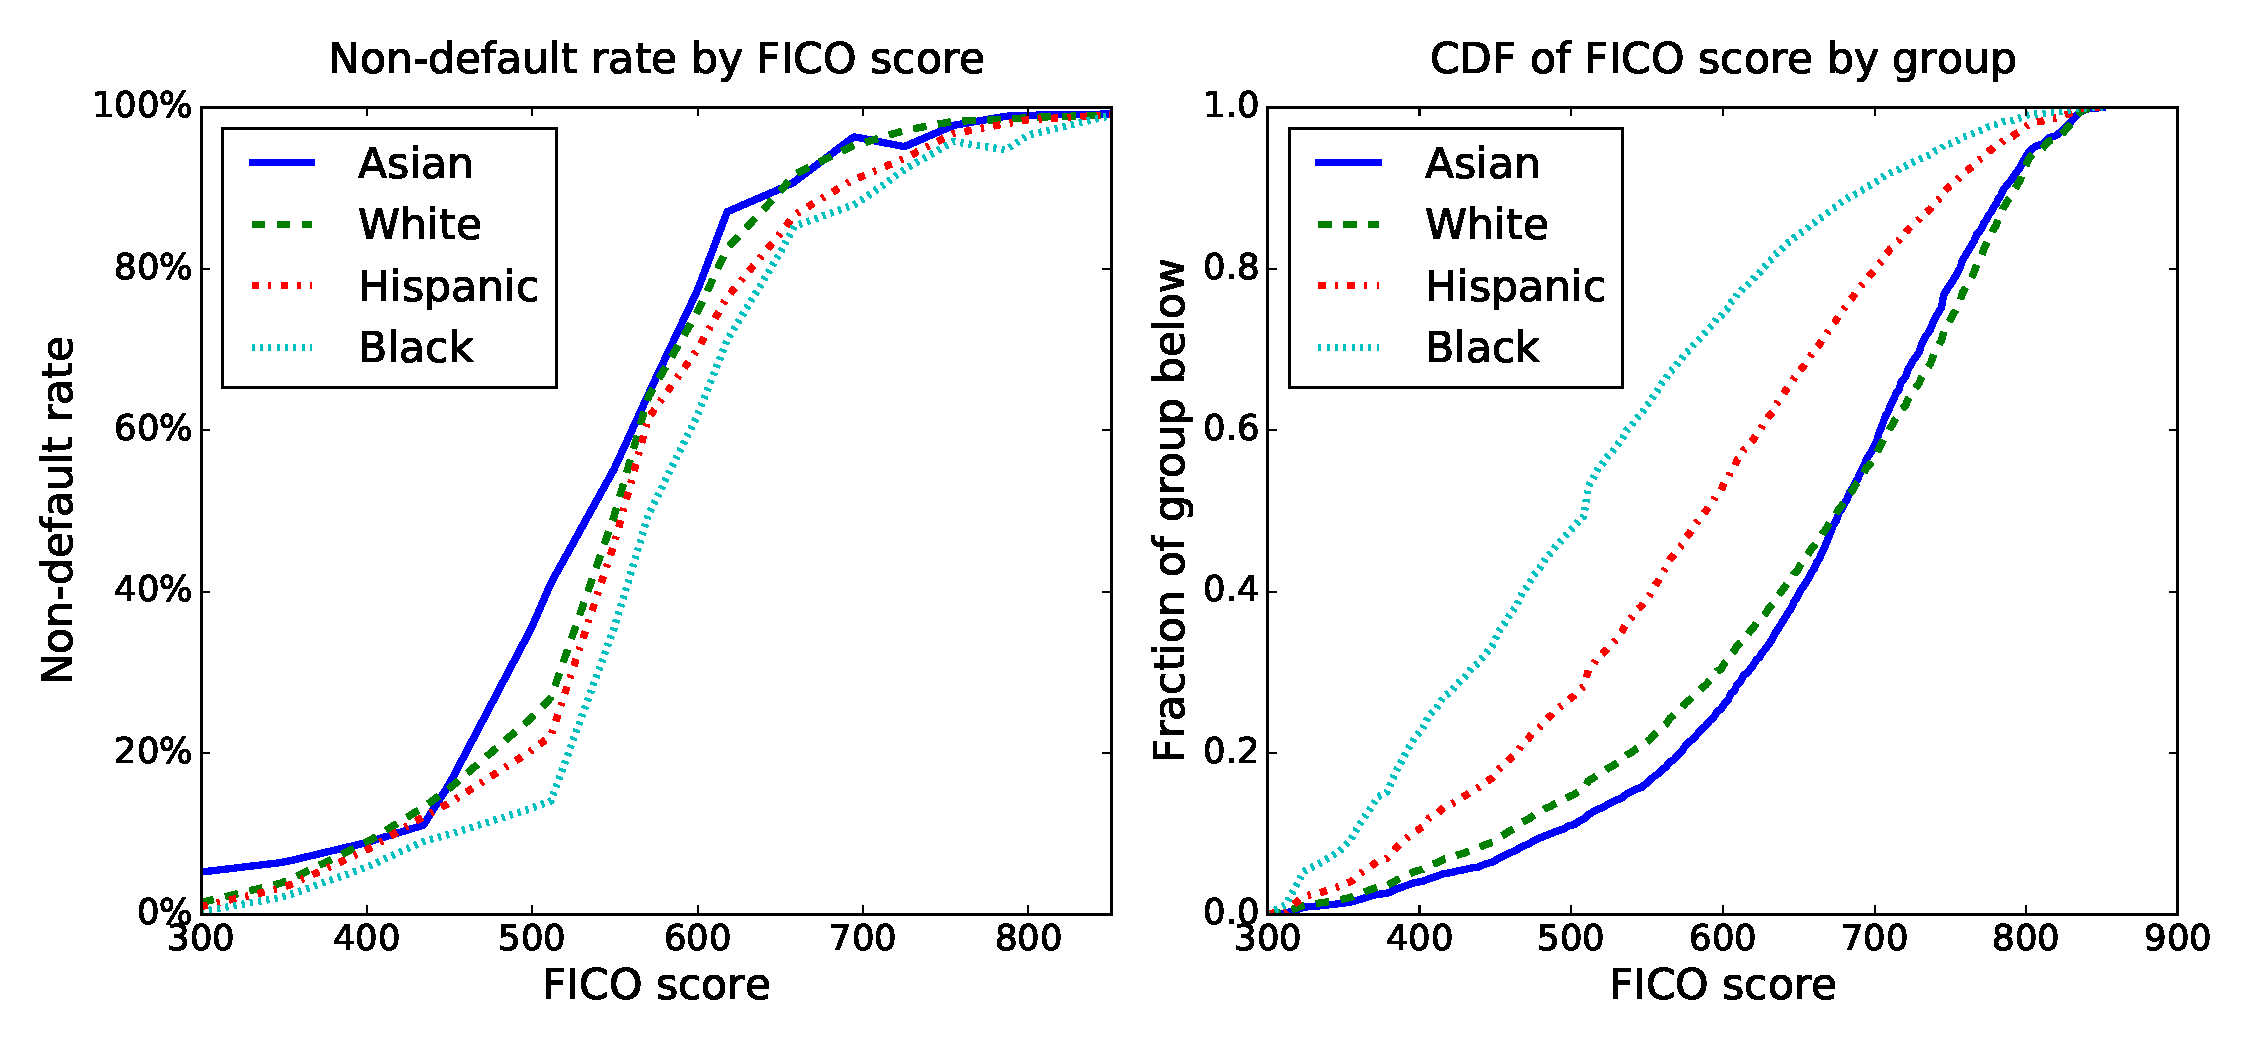
\includegraphics[width=\textwidth]{figs/fico-marginals}
  \caption{These two marginals, and the number of people per group,
    constitute our input data.}
  \label{fig:fico-marginals}
\end{figure}
A credit score cutoff of 620 is commonly used for prime-rate
loans\footnote{\url{http://www.creditscoring.com/pages/bar.htm}
  (Accessed: 2016-09-20)}, which corresponds to an any-account default
rate of 18\%.  Note that this measures default on \emph{any} account
TransUnion was aware of; it corresponds to a much lower ($\approx
2\%$) chance of default on individual new loans.  To illustrate the
concepts, we use any-account default as our target~$Y$---a higher
positive rate better illustrates the difference between equalized odds
and equal opportunity.


We therefore consider the behavior of a lender who makes money on
default rates below this, i.e., for whom whom false positives (giving
loans to people that default on any account) is 82/18 as expensive as
false negatives (not giving a loan to people that don't default). The
lender thus wants to construct a predictor $\Yhat$ that is optimal
with respect to this asymmetric loss.  A typical classifier will pick
a threshold per group and set $\Yhat = 1$ for people with FICO scores
above the threshold for their group.  Given the marginal distributions
for each group (Figure~\ref{fig:fico-marginals}), we can study the
optimal profit-maximizing classifier under five different constraints
on allowed predictors:
\begin{figure}
  \centering
  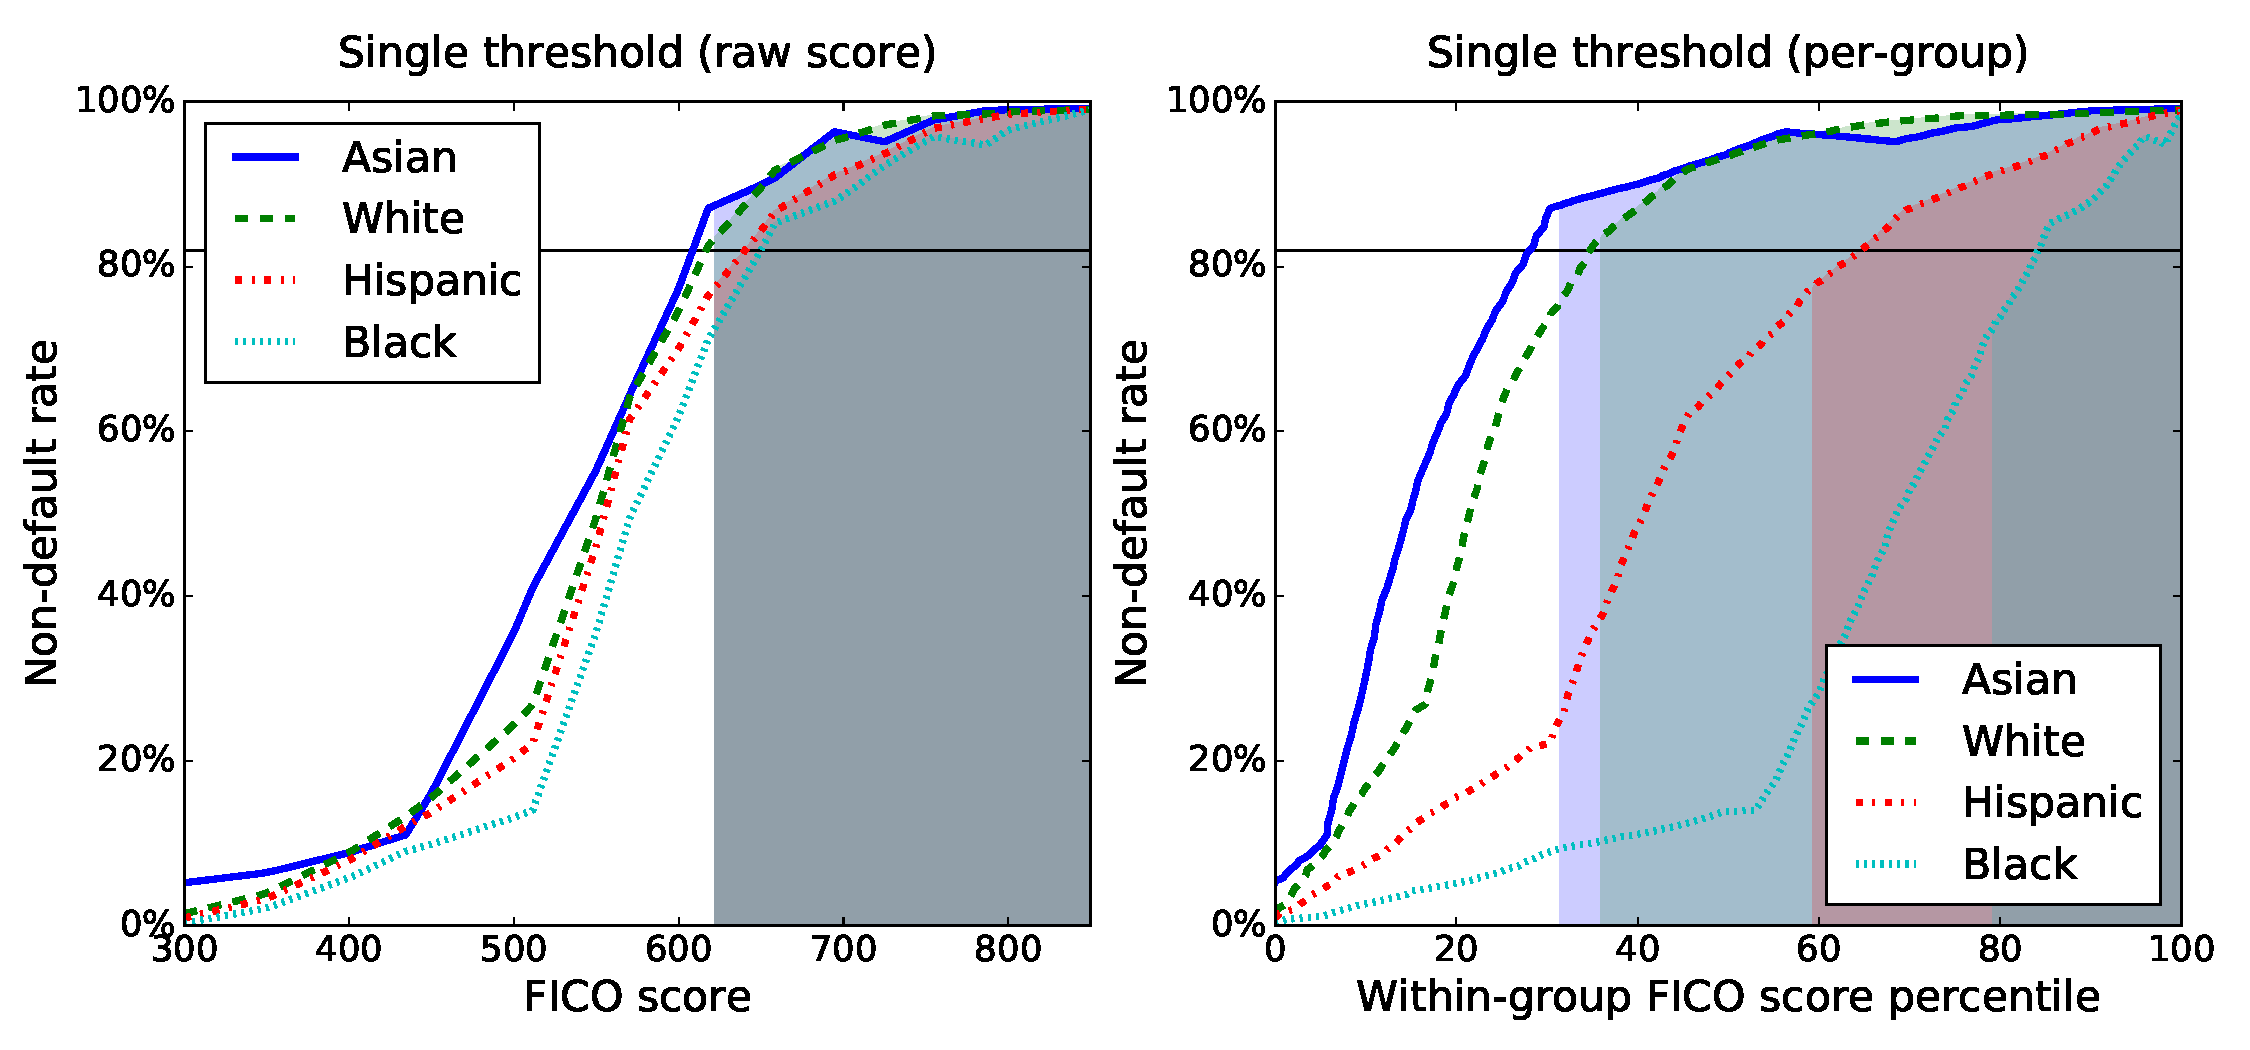
\includegraphics[width=0.9\textwidth]{figs/fico-fixed}
  \caption{The common FICO threshold of 620 corresponds to a
    non-default rate of 82\%.  Rescaling the $x$ axis to represent the
    within-group thresholds (right), $\Pr[\Yhat=1\mid Y=1,A]$ is the
    fraction of the area under the curve that is shaded. This means
    black non-defaulters are much less likely to qualify for loans
    than white or Asian ones, so a race blind score threshold violates
    our fairness definitions.}
  \label{fig:fico-fixed}
\end{figure}
%
\begin{itemize}
\item \textbf{Max profit} has no fairness constraints, and will pick
  for each group the threshold that maximizes profit.  This is the
  score at which 82\% of people in that group do not default.
\item \textbf{Race blind} requires the threshold to be the same for
  each group.  Hence it will pick the single threshold at which 82\%
  of people do not default overall, shown in
  Figure~\ref{fig:fico-fixed}.
\item \textbf{Demographic parity} picks for each group a threshold
  such that the fraction of group members that qualify for loans is the same.
\item \textbf{Equal opportunity} picks for each group a threshold such
  that the fraction of \emph{non-defaulting} group members that qualify for loans is the
  same.
\item \textbf{Equalized odds} requires both the fraction of non-defaulters
  that qualify for loans and the fraction of defaulters that qualify
  for loans to be constant across groups.  This cannot be achieved with
  a single threshold for each group, but requires randomization.
  There are many ways to do it; here, we pick \emph{two} thresholds
  for each group, so above both thresholds people always qualify and
  between the thresholds people qualify with some probability.
\end{itemize}
%
We could generalize the above constraints to allow non-threshold
classifiers, but we can show that each profit-maximizing classifier
will use thresholds. As shown in Section~\ref{sec:achieving}, the
optimal thresholds can be computed efficiently; the results are shown
in Figure~\ref{fig:fico-thresholds}.
%
\begin{figure}[h!]
  \centering
  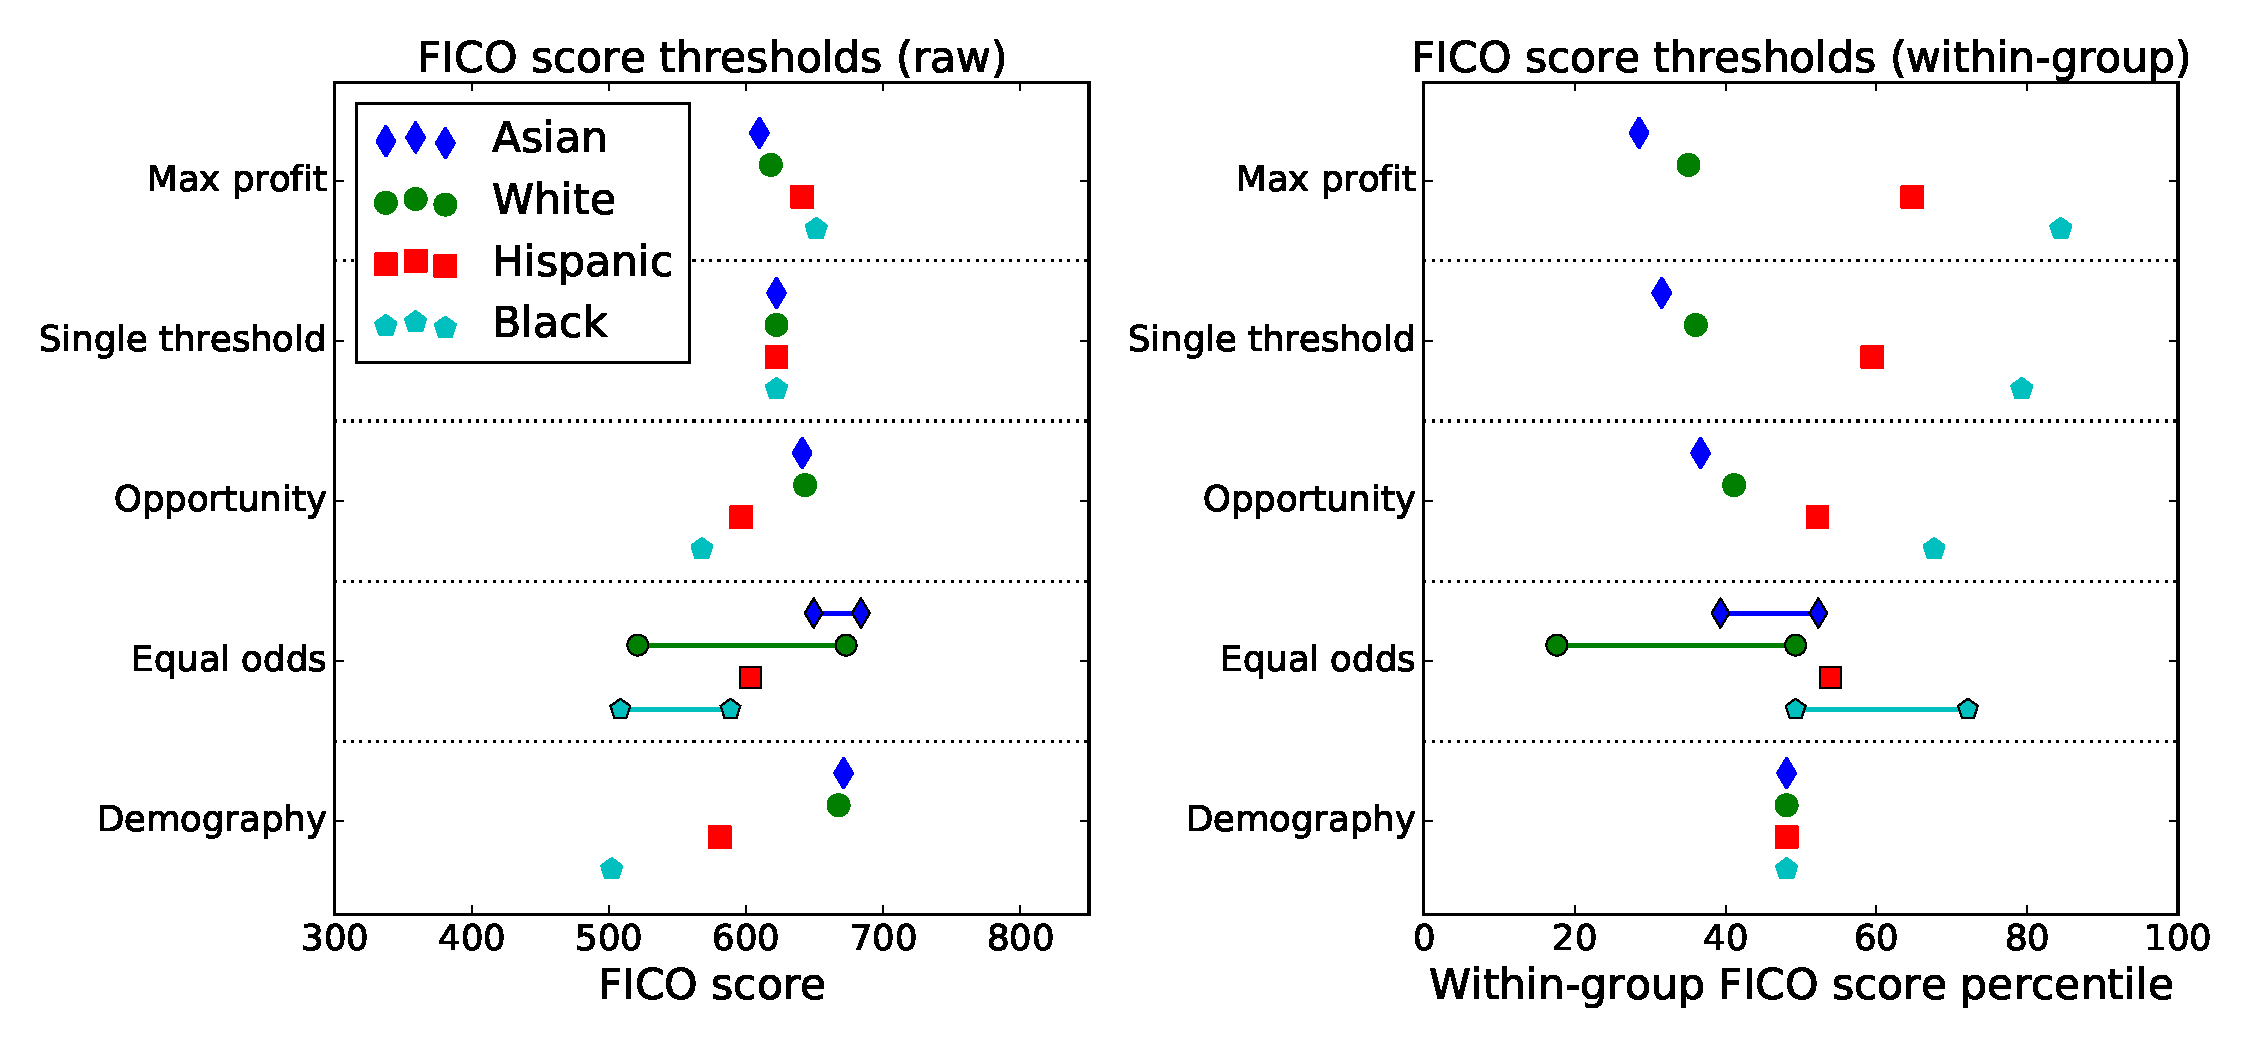
\includegraphics[width=\textwidth]{figs/fico-thresholds}
  \caption{FICO thresholds for various definitions of fairness.
    The equal odds method does not give a single
    threshold, but instead $\Pr[\Yhat = 1 \mid R,A]$ increases over some
    not uniquely defined range; we pick the one containing the fewest people.
    Observe that, within each race, the equal opportunity threshold
    and average equal odds threshold lie between the max profit
    threshold and equal demography thresholds.
  }
  \label{fig:fico-thresholds}
\end{figure}
%
Our proposed fairness
definitions give thresholds between those of max-profit/race-blind
thresholds and of demographic parity.
%
\begin{figure}
  \centering
  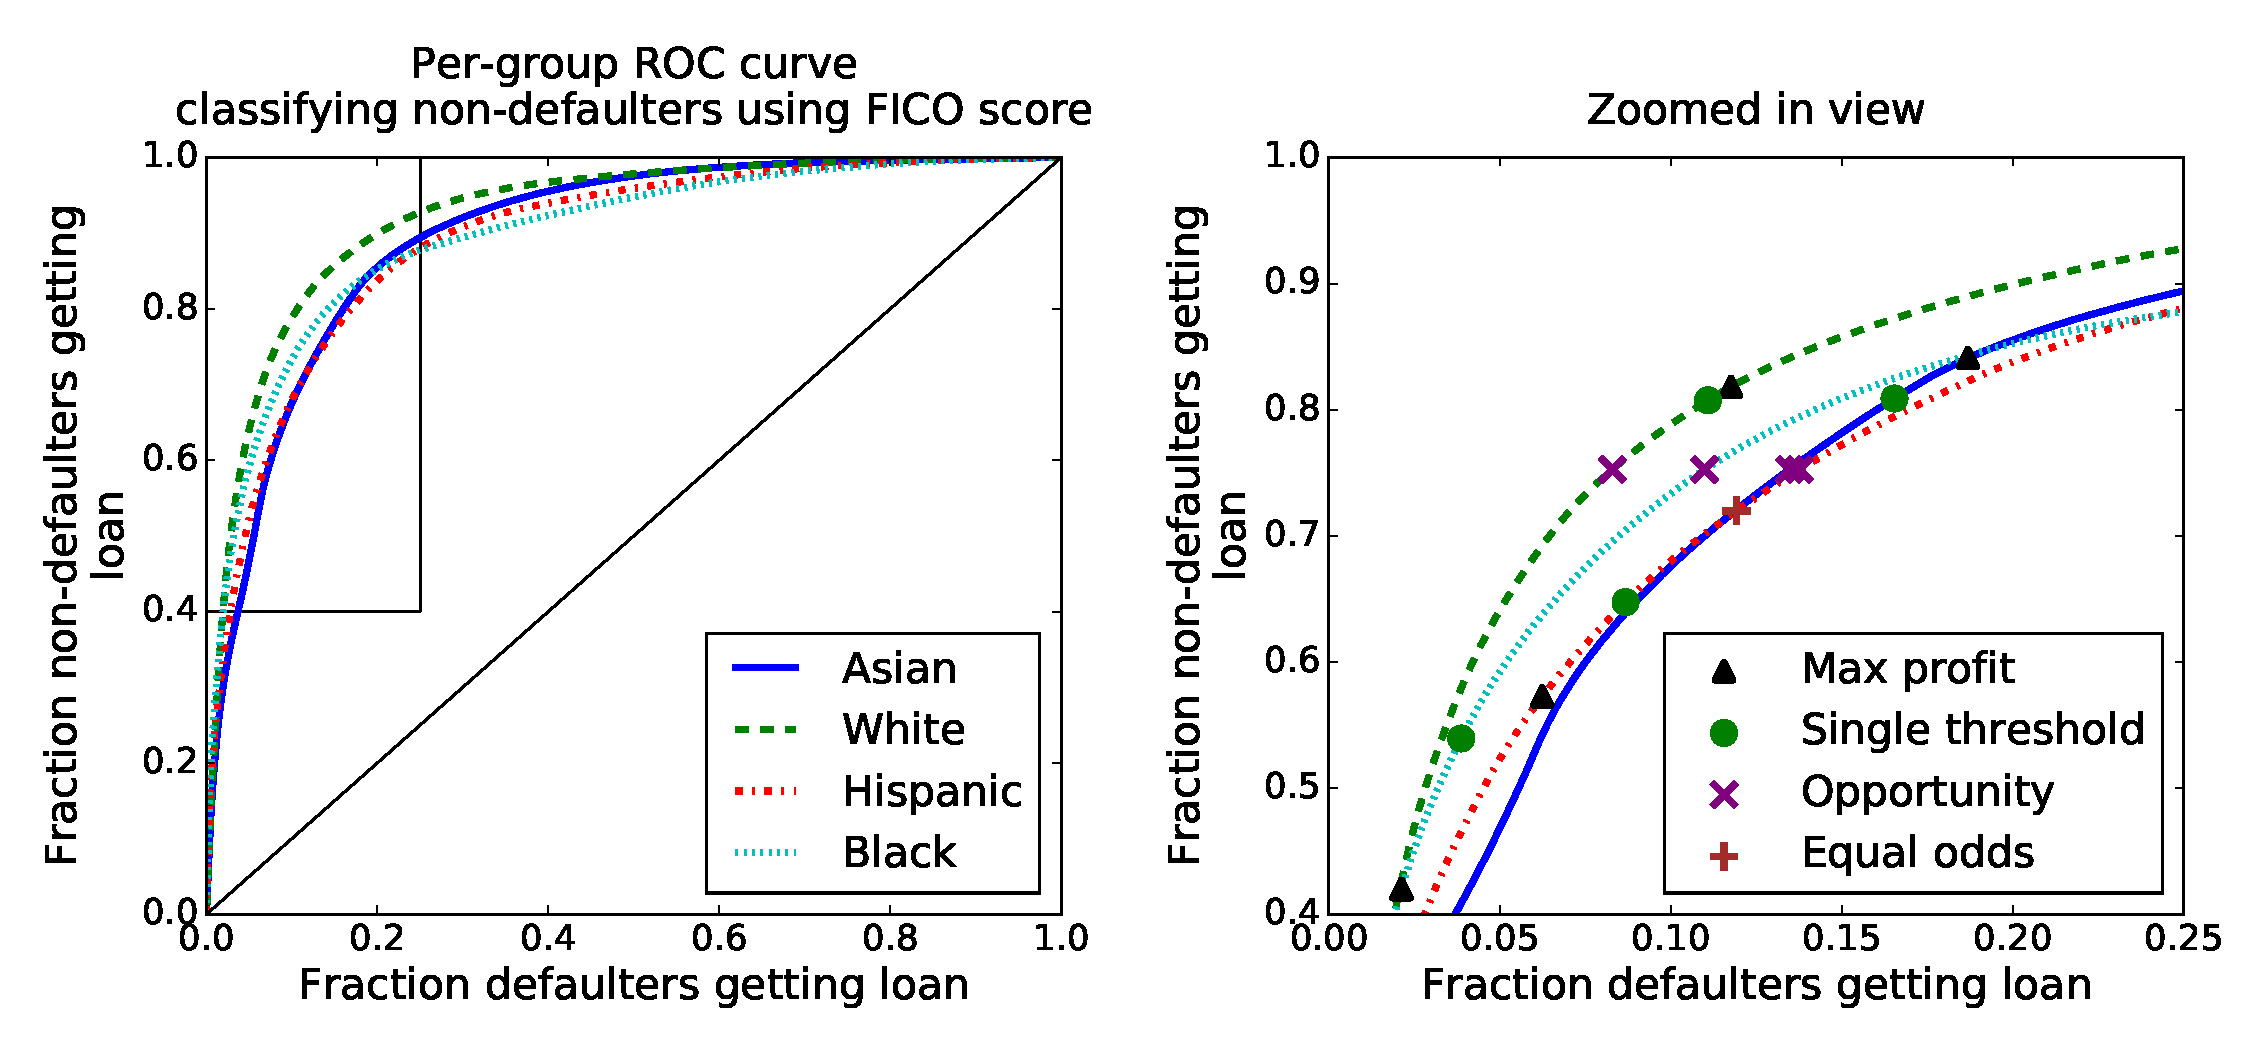
\includegraphics[width=\textwidth]{figs/fico-roc}
  \caption{The ROC curve for using FICO score to identify
    non-defaulters.  Within a group, we can achieve any convex
    combination of these outcomes.  Equality of opportunity picks
    points along the same horizontal line.  Equal odds picks a point
    below all lines.}
  \label{fig:fico-roc}
\end{figure}
%
Figure~\ref{fig:fico-roc} plots the ROC curves for each group.  It
should be emphasized that differences in the ROC curve do not indicate
differences in default behavior but rather differences in prediction
accuracy---lower curves indicate FICO scores are less predictive for
those populations.  This demonstrates, as one should expect, that the
majority (white) group is classified more accurately than minority
groups, even over-represented minority groups like Asians.

The left side of Figure~\ref{fig:fico-profit} shows the fraction of
people that wouldn't default that would qualify for loans by the
various metrics.  Under max-profit and race-blind thresholds, we find
that black people that would not default have a significantly harder
time qualifying for loans than others.  Under demographic parity, the
situation is reversed.
%
\begin{figure}[h!]
  \centering
  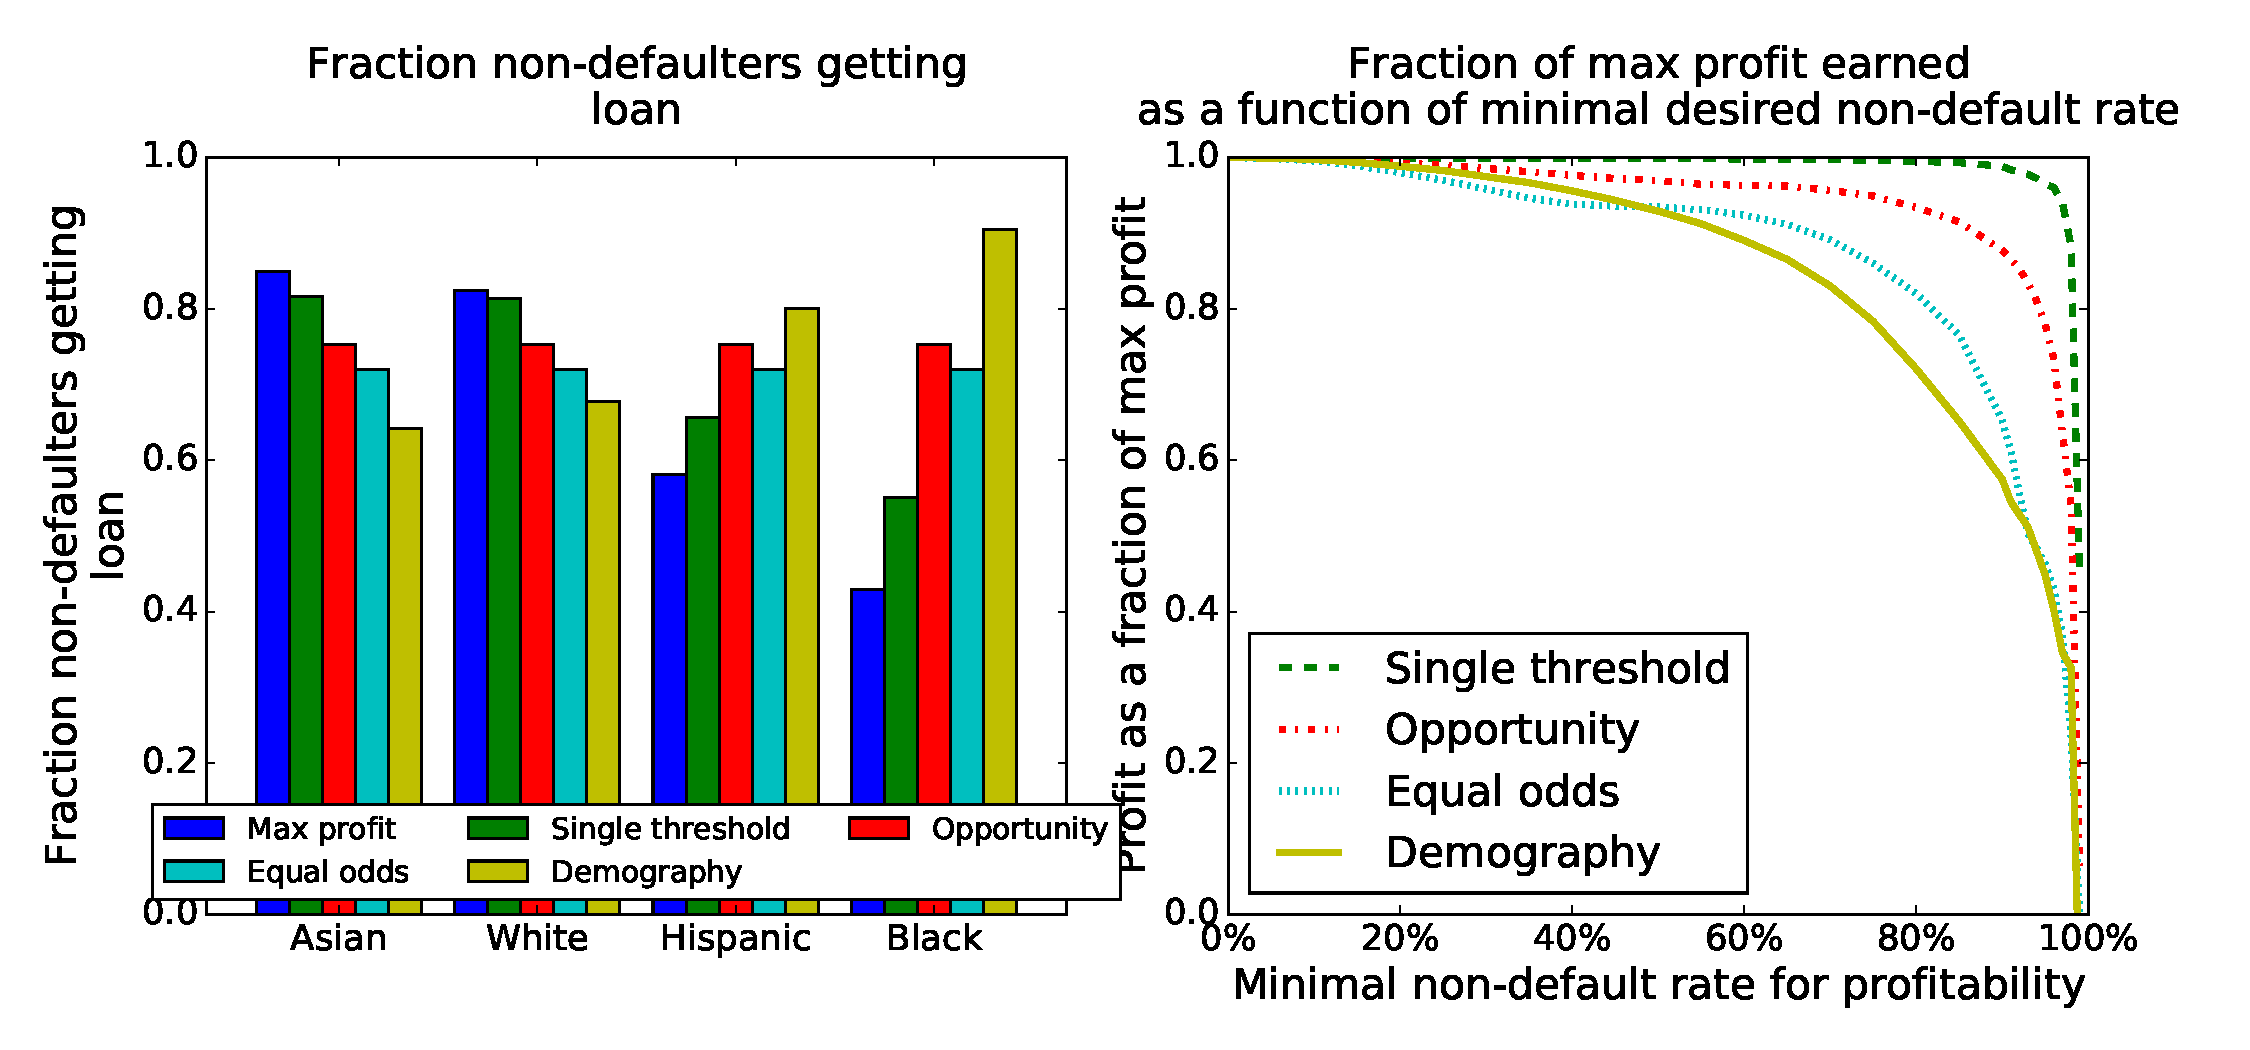
\includegraphics[width=\textwidth]{figs/fico-targets}
  \caption{On the left, we see the fraction of non-defaulters that
    would get loans.  On the right, we see the profit achievable for
    each notion of fairness, as a function of the false
    positive/negative trade-off.}
  \label{fig:fico-profit}
\end{figure}
%

The right side of Figure~\ref{fig:fico-profit} gives the profit
achieved by each method, as a fraction of the max profit achievable.
We show this as a function of the non-default rate above which loans
are profitable (i.e. 82\% in the other figures).  At 82\%, we find
that a race blind threshold gets 99.3\% of the maximal profit, equal
opportunity gets 92.8\%, equalized odds gets 80.2\%, and demographic
parity gets 69.8\%.  So equal opportunity fairness costs less than a
quarter what demographic parity costs---and if the classifier
improves, this would reduce further.

The difference between equal odds and equal opportunity is that under
equal opportunity, the classifier can make use of its better accuracy
among whites.  Under equal odds this is viewed as unfair, since it
means that white people who wouldn't pay their loans have a harder
time getting them than minorities who wouldn't pay their loans.  An
equal odds classifier must classify everyone as poorly as the hardest
group, which is why it costs over twice as much in this case.  This
also leads to more conservative lending, so it is slightly harder for
non-defaulters of all groups to get loans.

The equal opportunity classifier does make it easier for defaulters to
get loans if they are minorities, but the incentives are aligned properly.
Under max profit, a small group may not be worth figuring out how to
classify and so be treated poorly, since the classifier can't identify
the qualified individuals.  Under equal opportunity, such
poorly-classified groups are instead treated better than
well-classified groups.  The cost is thus born by the company using
the classifier, which can decide to invest in better classification,
rather than the classified group, which cannot.  Equalized odds gives
a similar, but much stronger, incentive since the cost for a small
group is not proportional to its size.

While race blindness achieves high profit, the fairness guarantee is
quite weak.  As with max profit, small groups may be classified poorly
and so treated poorly, and the company has little incentive to improve
the accuracy.  Furthermore, when race is redundantly encoded, race
blindness degenerates into max profit.
